\documentclass[11pt,letterpaper]{article}

\usepackage{threeparttable}
\usepackage{textcomp,marvosym}
\usepackage{amsmath,amssymb}
\usepackage[left]{lineno}
\usepackage{changepage}
\usepackage{rotating}
\usepackage{natbib}
\usepackage{setspace}
\usepackage{fancyhdr}
\usepackage{graphicx}
\usepackage{booktabs}
\usepackage{pdfpages}
\usepackage{url}
\usepackage{longtable}
\usepackage{pdflscape}
\usepackage[outercaption]{sidecap}
\doublespacing

\raggedright
\textwidth = 6.5 in
\textheight = 9 in
\oddsidemargin = 0.0 in
\evensidemargin = 0.0 in
\topmargin = 0.0 in
\headheight = 0.0 in
\headsep = 0.0 in
\parskip = 0.1 in
\parindent = 0.2 in

\usepackage[aboveskip=1pt,labelfont=bf,labelsep=period,justification=raggedright,singlelinecheck=off]{caption}

%commands that were used to generate a PDF that was copied to make the .docx version for GSAB
%\pagestyle{empty}
%\usepackage[nomarkers,figuresonly]{endfloat}

\begin{document}

\begin{flushleft}
{\Large \textbf{The Precambrian paleogeography of Laurentia}}
\\

Nicholas L. Swanson-Hysell\textsuperscript{1}

\bigskip

\textsuperscript{1} Department of Earth and Planetary Science, University of California, Berkeley, CA 94720 USA

\end{flushleft}

\noindent\textit{This chapter is in preparation for the book Ancient Supercontinents and the Paleogeography of the Earth}

%\linenumbers

\section*{INTRODUCTION}

Laurentia was a major continent throughout the majority of the Proterozoic and is hypothesized to have been a central constituent of both the Paleoproterozoic Nuna and Neoproterozoic Rodinia supercontinents. The paleogeographic position of Laurentia is key to the development of reconstructions of Proterozoic paleogeography. There is a rich record of Precambrian paleomagnetic poles from Laurentia that is key to evaluating and developing paleogeographic models.

Laurentia refers to the craton that forms the Precambrian core of North America. Laurentia is comprised of multiple Archean cratons that had unique histories prior to their amalgmation in the Paleoproterozoic, as well as tectonic zones of crustal growth that post-date this assembly \citep{Hoffman1988a, Whitmeyer2007a}. Collision between the Superior Craton and the composite Slave+Rae+Hearne+Nain cratons that resulted in the the Trans-Hudson orogeny represents a major event in the formation of Laurentia \citep{Corrigan2009a}. Terminal collison recorded in the Trans-Hudson orogeny is estimated to have been ca. 1.86 to 1.82 Ga based on constraints such as U-Pb dating of monazite grains and zircon rims \citep[e.g.]{Skipton2016a, Weller2017a}. A period of accretionary and collision orogenesis is recorded in the constituent cratons and terranes of Laurentia leading up to the terminal collison of the Trans-Hudson orogeny. Coeval with the Trans-Hudson orogeny was the perphiral Penokean orogeny on the southern margin of the Superior cratron with the last evidence of that orogeny being ca. 1.78 undeformed plutons of the East Central Minnesota Batholith \citep{Holm2005a}. This overall story of rapid Paleoproterozoic amalgamation of Laurentia's constituent cratons, including the terminal Trans-Hudson orogeny, was synthesized in the seminal paper \textit{United Plates of America} \citep{Hoffman1988a} and has been refined in the time since -- particularly with additional geochronological constraints. Of most relevance here, are the events that led to the suturing of the more major cratonic blocks: the Thelon orogeny associated with the collision between the Slave craton and the Rae craton ca. 2.0 to 1.9 Ga (Hoffman, 1988); the Snowbird orogeny associated with ca. 1.89 Ga collision between the Rae and Hearne cratons and associated terranes (Berman et al., 2007); the XXXXXX orogeny associated with ca. 1.86 Ga collision between the Rae and Nain cratons (St-Onge et al., 2009). As for the Wyoming craton, many models posit that it was conjoined with Hearne and associated cratons as the time of the Trans-Hudson orogeny (e.g. St-Onge et al., 2009; Pehrsson et al., 2015) although a contrasting view has been been proposed that it arrived ca. 1.72 Ga after the accretionary Yavapai and Penokean orogenies (Kilian et al. 2016).  

In the paleogeographic model framework of \cite{Pehrsson2015a}, the cratonic and terrane collisions leading up to the Trans-Hudson orogeny mark the initial phase of assembly of the supercontinent Nuna. The Trans-Hudson orogeny itself is taken to be the terminal collision associated with the closure of the Manikewan Ocean that had previous been a large oceanic tract separating the Superior craton from the composite Slave+Rae+Hearne+Nain cratons (often referred to as the Churchill domain or plate; e.g. \citealp{Skipton2016a, Weller2017a}. This model posits that this period terminal collision is not only associated with the amalgmation of Laurentia, but is also associated with the assembly of the supercontinent Nuna that including other major Paleoproterozoic cratons including Siberia, Congo/Sao Francisco, West Africa, and Amazonia \citep{Pehrsson2015a}. Following the Trans-Hudson orogeny, the locus of orogenesis migrated to the exterior of Laurentia. This change marks a change in the style of Laurentia's growth as subsequent growth proceeding dominantly through accretion of juvenile crust along the southern and eastern margin of the nucleus of Archean cratons (\citealp{Whitmeyer2007a}; \ref{fig:Laurentia_map}). Major growth of Laurentia following the amalgmation of these Archean cratons occured associated with the arc-continent collision of the ca. 1.71 to 1.68 Ga Yavapai orogeny whose accretion was followed by widespread emplacement of granitoid intrusions \citep{Whitmeyer2007a}. These intrusions are hypothesized to have stablized the juvenile accreted terranes that subsequently remained part of Laurentia \citep{Whitmeyer2007a}. Subsequent accretionary orogenesis of the ca. 1.65–1.60 Ga Mazatzal Orogeny and associated plutonism lead to further crustal growth in the latest Paleoproterozoic. Laurentia's growth continued in the Mesoproterozoic along the southeast margin through further juvenile terrane and arc accretion. An interval of major plutonism occured ca. 1.48–1.35 Ga leading to the formation of A-type granitoids throughout both Mesoproterozoic and Paleoproterozoic provinces. In the latest Mesoproterozoic ca. 1.11-1.08 Ga, a major intracontinental rift co-located with the a large igneous province formed in Laurentia's interior leading to extension within the Archean Superior craton and Paleoproterozoic provinces. This Midcontinent Rfit lead to the formation of a thick succession of volcanics and mafic intrusions that are well-preserved in Laurentia's interior.  Midcontinent Rift development ceased as major collisional orogenesis of the Grenvillian orogeny began \citep{Swanson-Hysell2019a}. The Grenvillian orogeny was a protracted interval of continent-continent collision (ca. 1.09 to 0.98 Ga) which is interpreted to have resulted in the development of a thick orogenic plateau \citep{Rivers2008a} and is typically to interpretted to have been a major collisional event associated with the amalgamation of continents into the supercontinent Rodinia \citep{Hoffman1991a}.




\begin{figure}
\centering
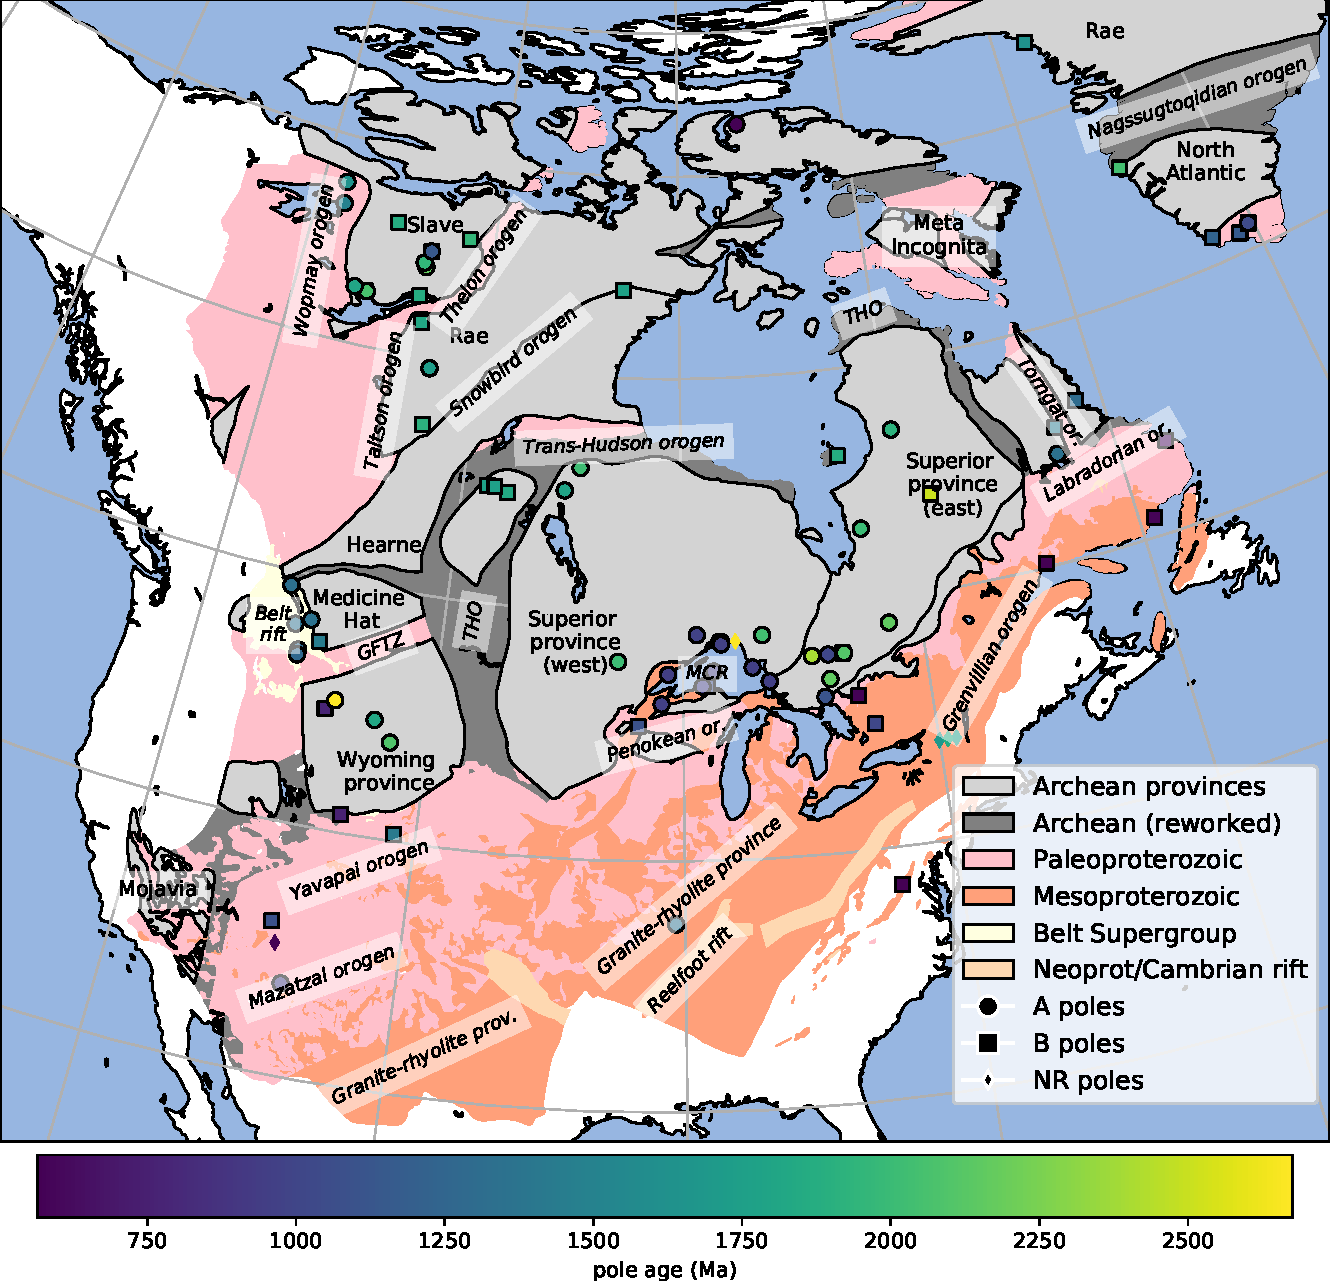
\includegraphics[width=6.5 in]{Figures/Fig1_map.pdf}
\caption{\small{\textbf{Simplified map of Laurentia showing the location of Archean cratons (labeled with text) and younger Paleoproterozoic and Mesoproterozoic crust (simplified from \cite{Whitmeyer2007a}). The localities from which the compiled Precambrian paleomagnetic poles were developed are shown and colored by age. The circles (A rated poles) and squares (B rated poles) have been assessed by the Nordic workshop panel while the diamonds are additional not-rated results from the Paleomagia database.}}}
\label{fig:Laurentia_map}
\end{figure}

\section{Paleomagnetic pole compilation}

This chapter utilizes the compilation of paleomagnetic poles developed through the Nordic Paleomagnetism Workshops with some additions and modifications. The Nordic Paleomagnetism Workshops have taken the approach of using expert panels to assess paleomagnetic poles and assign them grades meant to convey the confidence that the community has in these results. While many factors associated with paleomagnetic poles can be assessed quantitatively such as the Fisher statistics and the precision of geochronological constraints, other aspects such as the degree to which available field tests constrain the magnetization to be primary require expert assessment. The categorizations used by the expert panel are `A' and `B' with the last panel meeting occuring in Fall 2017 in Leirubakki, Iceland. An `A' rating refers to poles that are judged to be of such high-quality that they provide essential constraints that should be satisfied in paleogeographic reconstructions. A `B' rating is associated with poles that are judged to likely provide a high-quality constraint, but have some deficiency such as remaining ambiguity in the demonstration of primary remanence or the quality/precision of available geochronologic constraints. Additional poles that were not given an `A' or `B' classification at the Nordic Workshops are referred to as not-rated (`NR').

Prior to the termination of the Trans-Hudson orogeny (before 1.8 Ga), we consider paleomagnetic poles with respect to the individual Archean cratons. There are poles in the compilation for the Slave, Wyoming, Rae, Superior and Nain cratons. Following the termination of this orogeny (after 1.8 Ga), we consider poles from all the respective cratons and terranes to reflect the position of all of Laurentia.

For the Superior craton, an additional complexity is that paleomagnetic poles from Siderian to Rhyacian Period (2.50 to 2.05 Ga) dike swarms, as well as deflection of dike trends, support an interpretation that there as substantial Paleoproterozoic rotation of the western Superior craton relative to the eastern Superior craton across the Kapuskasing Structural Zone \citep{Bates1991a, Evans2010a}. \cite{Evans2010a} propose an Euler rotation of (51º N, 85º W, −14º CCW) to reconstruct western Superior relative to eastern Superior and interpret that the rotation occured in the time interval of 2.07 to 1.87 Ga. I follow this interpretation and group the poles into Superior (West) and Superior (East). These poles are shown in Table 1 both in their initial reference frame and rotated into the other Superior reference frame.

Following Laurentia's amalgamation, poles from each part of the Laurentia can be considered to reflect the position of the entire composite craton. It is worth considering the possibility that poles from zones of Paleoproterozoic and Mesoproterozoic accretion could be allochthonous to the craton. \cite{Hall201Xa} argued that this was the case for late Mesoproterozoic and early Neoproterozoic poles from east of the Grenvillian allochothon boundary fault. However, the majority of researchers have considered these poles to post-date major differential motion and be associated with cooling during collapse of thick plateau developed during continent-continent collision (e.g. \cite{}). Poles are also included in the composite that come from terranes that were once part of Laurentia, but have subsequently rifted away. These poles need to be rotated into the Laurentia reference frame prior to use for tectonic reconstruction.
\begin{itemize}
\item Laurentia-Greenland.  1202 1800.0   67.5 -118.5  -13.8  1000 !Rotation of Greenland to Laurentia
\item Laurentia-Scotland 1022 1800.0   73.0   96.5  -22.0  1000 !Rotate (proto-)Scotland to Laurentia-Greenland fit according to Darabi2004
\item Laurentia-Svalbard 3301 1275.0  -81.0  125.0   68.0  1000 !Rotate Svalbard to Laurentia in fit that works well with East Greenland basin (Maloof et al., 2006 rotation)
\end{itemize}

\end{{document}